% Exam Template for UMTYMP and Math Department courses
%
% Using Philip Hirschhorn's exam.cls: http://www-math.mit.edu/~psh/#ExamCls
%
% run pdflatex on a finished exam at least three times to do the grading table on front page.
%
%%%%%%%%%%%%%%%%%%%%%%%%%%%%%%%%%%%%%%%%%%%%%%%%%%%%%%%%%%%%%%%%%%%%%%%%%%%%%%%%%%%%%%%%%%%%%%

% These lines can probably stay unchanged, although you can remove the last
% two packages if you're not making pictures with tikz.
\documentclass[11pt]{exam}
\RequirePackage{amssymb, amsfonts, amsmath, latexsym, verbatim, xspace, setspace}
\RequirePackage{tikz, pgflibraryplotmarks}

% By default LaTeX uses large margins.  This doesn't work well on exams; problems
% end up in the "middle" of the page, reducing the amount of space for students
% to work on them.
\usepackage[margin=1in]{geometry}
\usepackage{afterpage}

\usepackage{url}
% Here's where you edit the Class, Exam, Date, etc.
\newcommand{\class}{CS/EE 3810}
\newcommand{\term}{Fall 2022}
\newcommand{\examnum}{Midterm}
\newcommand{\examdate}{10/24/2022}
\newcommand{\timelimit}{11:50am - 1:10pm}

% For an exam, single spacing is most appropriate
\singlespacing
% \onehalfspacing
% \doublespacing

% For an exam, we generally want to turn off paragraph indentation
\parindent 0ex

\begin{document} 

% These commands set up the running header on the top of the exam pages
\pagestyle{head}
\firstpageheader{}{}{}
\runningheader{\class}{\examnum\ - Page \thepage\ of
\numpages}{\fbox{\rule{2in}{0pt}\rule[-0.5ex]{0pt}{5ex}}}
\runningheadrule

\begin{flushright}
\begin{tabular}{p{2.8in} r l}
%\textbf{\class} & \textbf{Name (Print):} & \makebox[2in]{\hrulefill}\\
  \textbf{\class} & \textbf{Name (Print):} &
  \fbox{\rule{2in}{0pt}\rule[-0.5ex]{0pt}{5ex}}\\
   \textbf{\term} & \textbf{uid:} &
    \fbox{\parbox{0pt}{}\rule{2in}{0pt}\rule[-0.5ex]{0pt}{5ex}}\\
\textbf{\examnum} & \textbf{Left person:} &
    \fbox{\rule{2in}{0pt}\rule[-0.5ex]{0pt}{5ex}}\\
\textbf{\examdate} & \textbf{Right person:} &
    \fbox{\rule{2in}{0pt}\rule[-0.5ex]{0pt}{5ex}}\\
\textbf{Time Limit: \timelimit} & & \\
\end{tabular}\\
\end{flushright}
\rule[1ex]{\textwidth}{.1pt}




%\begin{minipage}[t]{3.7in}
%\vspace{0pt}
\begin{itemize}

\item \textbf{Don't forget to write your name on this exam.} 

\item \textbf{This is an open book, open notes exam. But no online or 
    in-class chatting.  } 

    
\item \textbf{Ask us if something is confusing in the questions.}

\item \textbf{Organize your work}, in a reasonably neat and coherent way, in
the space provided. Work scattered all over the page without a clear ordering will 
receive very little credit.  

\item \textbf{Mysterious or unsupported answers will not receive full
credit}.  A correct answer, unsupported by explanation will receive no credit; 
an incorrect answer supported by substantially correct explanations might still 
receive partial credit.

\item If you need more space, use the back of the pages; clearly indicate when you have done this.
\end{itemize}

%Do not write in the table to the right.
%\end{minipage}
%\hfill

%\begin{minipage}[t]{2.3in}
%\vspace{0pt}
%\cellwidth{3em}
%\gradetablestretch{2}
\vqword{Problem}
\addpoints % required here by exam.cls, even though questions haven't started yet.	
\gradetable[v]%[pages]  % Use [pages] to have grading table by page instead of question

%\end{minipage}
\newpage % End of cover page

%%%%%%%%%%%%%%%%%%%%%%%%%%%%%%%%%%%%%%%%%%%%%%%%%%%%%%%%%%%%%%%%%%%%%%%%%%%%%%%%%%%%%
%
% See http://www-math.mit.edu/~psh/#ExamCls for full documentation, but the questions
% below give an idea of how to write questions [with parts] and have the points
% tracked automatically on the cover page.
%
%
%%%%%%%%%%%%%%%%%%%%%%%%%%%%%%%%%%%%%%%%%%%%%%%%%%%%%%%%%%%%%%%%%%%%%%%%%%%%%%%%%%%%%

\begin{questions}

\addpoints
\question Performance equation

Compilers can have a profound impact on the performance
of an application. Assume that for a program, compiler A results in a dynamic
	instruction count of 1.0E9 (i.e., counted by the CPU with a hardware performance counter
	during execution of the 
	program) and has an execution time of 1.1 s, while compiler B
results in a dynamic instruction count of 1.2E9 and an execution time of 1.5 s.

	
\begin{parts}
 
\part[10] 


Find the average CPI for each program given that the processor has a clock cycle
time of 1 ns.

\textbf{Answer:} We know that,

	$CPU time = Instruction count × CPI × Clock cycle time$

So,

$CPI = CPU time / (Instruction count × Clock cycle time)$

Compiler A:

	$CPI = 1.1 / (1.0E9 × 1.0E-9) = 1.1$

Compiler B:

	$CPI = 1.5 / (1.2E9 × 1.0E-9) = 1.25$

\vfill

\part[10]

Assume the compiled programs run on two different processors. If the execution
	times on the two processors are the same, how much faster is the clock
	of the processor running compiler A’s code versus the clock of the
	processor running compiler B’s code?

\textbf{Answer:}
We know that,
$1/ Clock cycle time = Instruction count × CPI / CPU time$

So,

	$Clock rate (Frequency) = Instruction count × CPI / CPU time$

For the same CPU or execution time on both processors (here we assume that CPI of each program stays the same as in part above),

$fB/fA = (Instruction count(B) × CPI(B)) / (Instruction count (A) × CPI(A))
= (1.2E9 × 1.25) / 1.0E9 × 1.1)
= 1.36$

\vfill


\end{parts}

\newpage
% Basic question
\addpoints
\question MIPS assembly 

\begin{parts}
 
\part[5] 

Which address is accessed by the following \texttt{lw} instruction, \texttt{\$s0} contains 1234? 
	
\begin{verbatim}
lw $s0, 4000($s0)
\end{verbatim}

\textbf{Answer:} $4000 + 1234 = 5234$ 

\vfill

\part[5] 

The address field of the jump (\texttt{j}) instruction contains 1234? What is
	the value of the \texttt{pc} (program counter) register after this jump
	instruction is executed? The initial value of the \texttt{pc} is
	2147483648.

\textbf{Answer:} We will take a simple answer $1234*4 = 4936$, but will give
	extra 5 points for mentioning that \texttt{j} uses \emph{pseudodirect}
	addressing which means that the top 4 bits of the PC are not changed,
	hence the address is $2147488584$. 

\vfill



\part[5] 

The address field of the branch when equal (\texttt{beq}) instruction contains 1234, and the value of the program couner is 4000. 
	What is the value of the \texttt{pc} (program counter) register after this \texttt{beq} instruction is executed (assume the condition 
	is true and the branch is taken)? 

\textbf{Answer:} $4000 + 4 + 1234*4 = 8940$

	
\vfill

\newpage

\part[10] Below is the source code a simple C program translate it into MIPS
	assembly (assume \texttt{a} is in \texttt{t0}, \texttt{b} is in
	\texttt{t1}, \texttt{c} is in \texttt{t2}, \texttt{d} is in
	\texttt{t3}, \texttt{e} is in \texttt{t4}, and \texttt{f} should be in
	\texttt{s0}. 

\begin{verbatim}
f = foo(a, b, c, d, e);
\end{verbatim}

I.e., you only have to write assembly for calling the function and getting the
	result back (you don't really care what the function is doing). 

However, you need to know the signature of the function, \texttt{foo} function
	takes 5 integers and returns an integer, i.e.: 

\begin{verbatim}
int foo(int a, int b, int c, int d, int e); 
\end{verbatim}

\textbf{Answer:} 


\begin{verbatim}

mov $a0, $t0      # first 4 arguments are in registers
mov $a1, $t1
mov $a2, $t2
mov $a3, $t3
addi $sp, $sp, -4 # stack grows down
sw $t4, $sp       # 5th arg is on the stack
jal foo
mov $s0, $v0
addi $sp, $sp, 4  # restore the stack

\end{verbatim}

\vfill


\newpage \part[20] Below is the source code a simple C program translate it
	into MIPS assembly

\begin{verbatim}
 int foo(int a) {               
         int sum = 0; 
          for (int i = 0; i < a; i++) 
             sum = sum + i;
         return sum;                
 }                                
                                  
 int bar(int n)      
 {                      
     return foo(n);             
 }                              
                                

\end{verbatim}

\textbf{Answer:} 

\begin{verbatim}
foo: 
        # this is a leaf function, no need to save/restore $ra
        move $v0, $zero         # sum is in $v0
        move $t0, $zero         # i is in $t0

  forloop:
        slt $t1, $t0, $a0       # set $t1 to 1 if $t0 is less then $a0 (i < n)
        beq $t1, $zero, exit    # $t1 is 0 (not set) only when i >= n

        add $v0, $v0, $t0       # sum = sum + i

        addi $t0, $t0, 1        # i += 1
        j forloop
  exit:
        jr $ra                  # return, sum is already in $v0  

bar: 
    addi $sp, $sp, -4 # stack grows down (reserve space for $ra)
    sw $ra, $sp       # save $ra
    jal foo           # call foo
    lw $ra, $sp       # restore $ra
    addi $sp, $sp, 4  # restore stack
    jr $ra            # return
    
\end{verbatim}


\vfill

\end{parts}

\newpage

\addpoints 

\question Linking and loading: relocation

Alice compiles the following C file. 

\begin{verbatim}
#include<stdio.h>

int add (int a, int b) {
    printf("Numbers are added together\n");
    return a+b;
}

int main() {
    int a,b;
    a = 3;
    b = 4;

    int ret = add(a,b);

    printf("Result: %u\n", ret);
    return 0; 
}
\end{verbatim}


\begin{parts}


\part[10] Which symbols need to be relocated? Note, that C treats string constants as globals allocated in the read-only 
	data section. Explain your answer. 

\begin{verbatim}
#include<stdio.h>

int add (int a, int b) {
    printf("Numbers are added together\n"); # access to string in the data section 
                                            # requires relocation, 
                                            # i.e., move $a0, <str_addr>
    return a+b;
}

int main() {
    int a,b;                                # a and b are local (on the stack or 
                                            # in registers
    a = 3;                                  # no need to relocate
    b = 4;

    int ret = add(a,b);                     # invocation of a function "add" (i.e., 
                                            # jal <some addr>)
                                            # ret is local (on the stack or in 
                                            # registers)

    printf("Result: %u\n", ret);            # access to string (move $a0, <str_addr> 
    return 0; 
}
\end{verbatim}




\vfill


\end{parts}

\newpage

\addpoints 

\question Floating point

\begin{parts}

\part[10] Provide an example of two IEEE 754 single precision floating point numbers and an operation on them which results in an \emph{overflow} when performed. 

\textbf{Answer:} Overflow occurs when a positive exponent becomes too large to fit in the exponent field.

Note that we cannot pick exponent to be 255 (all 1 in binary) since it represents NaN, so let's pick to floating points with exponents of 254 and a fraction of 
all 0. This represents a floating point number that is $1 * 2^{127}$ (here we assume that the sign is 0). If we multiply two such numbers the overflow occurs since the
exponent that is 127 + 127 + BIAS = 381 does not fit in the exponent field.   


\vfill
	

\part[10] Provide an example of two IEEE 754 single precision floating point numbers and an operation on them which results in \emph{rounding} when performed. 
	
\textbf{Answer:} Rounding is required when the fraction of the floating point number does not fit into the 23 bits allocated to store it (for single precision). 

Again we should be careful and avoid picking a floating point number with exponent of 0 as it represents a denormalized number. We therefore pick two numbers that 
have 1 as exponent and all 23 bits as 1 in the fraction field. Adding these two numbers will result in a fraction that is one bit larger than the fraction field, hence 
ronding is required. 

\vfill


\end{parts}


\newpage

\addpoints 

\question Data path

Use the figure below to explain execution of the branch on equal (\texttt{beq})
instruction in the MIPS datapath. 

\begin{figure}[h] \centering
%\includegraphics[width=1.0\columnwidth]{figs/shared-state.png}
	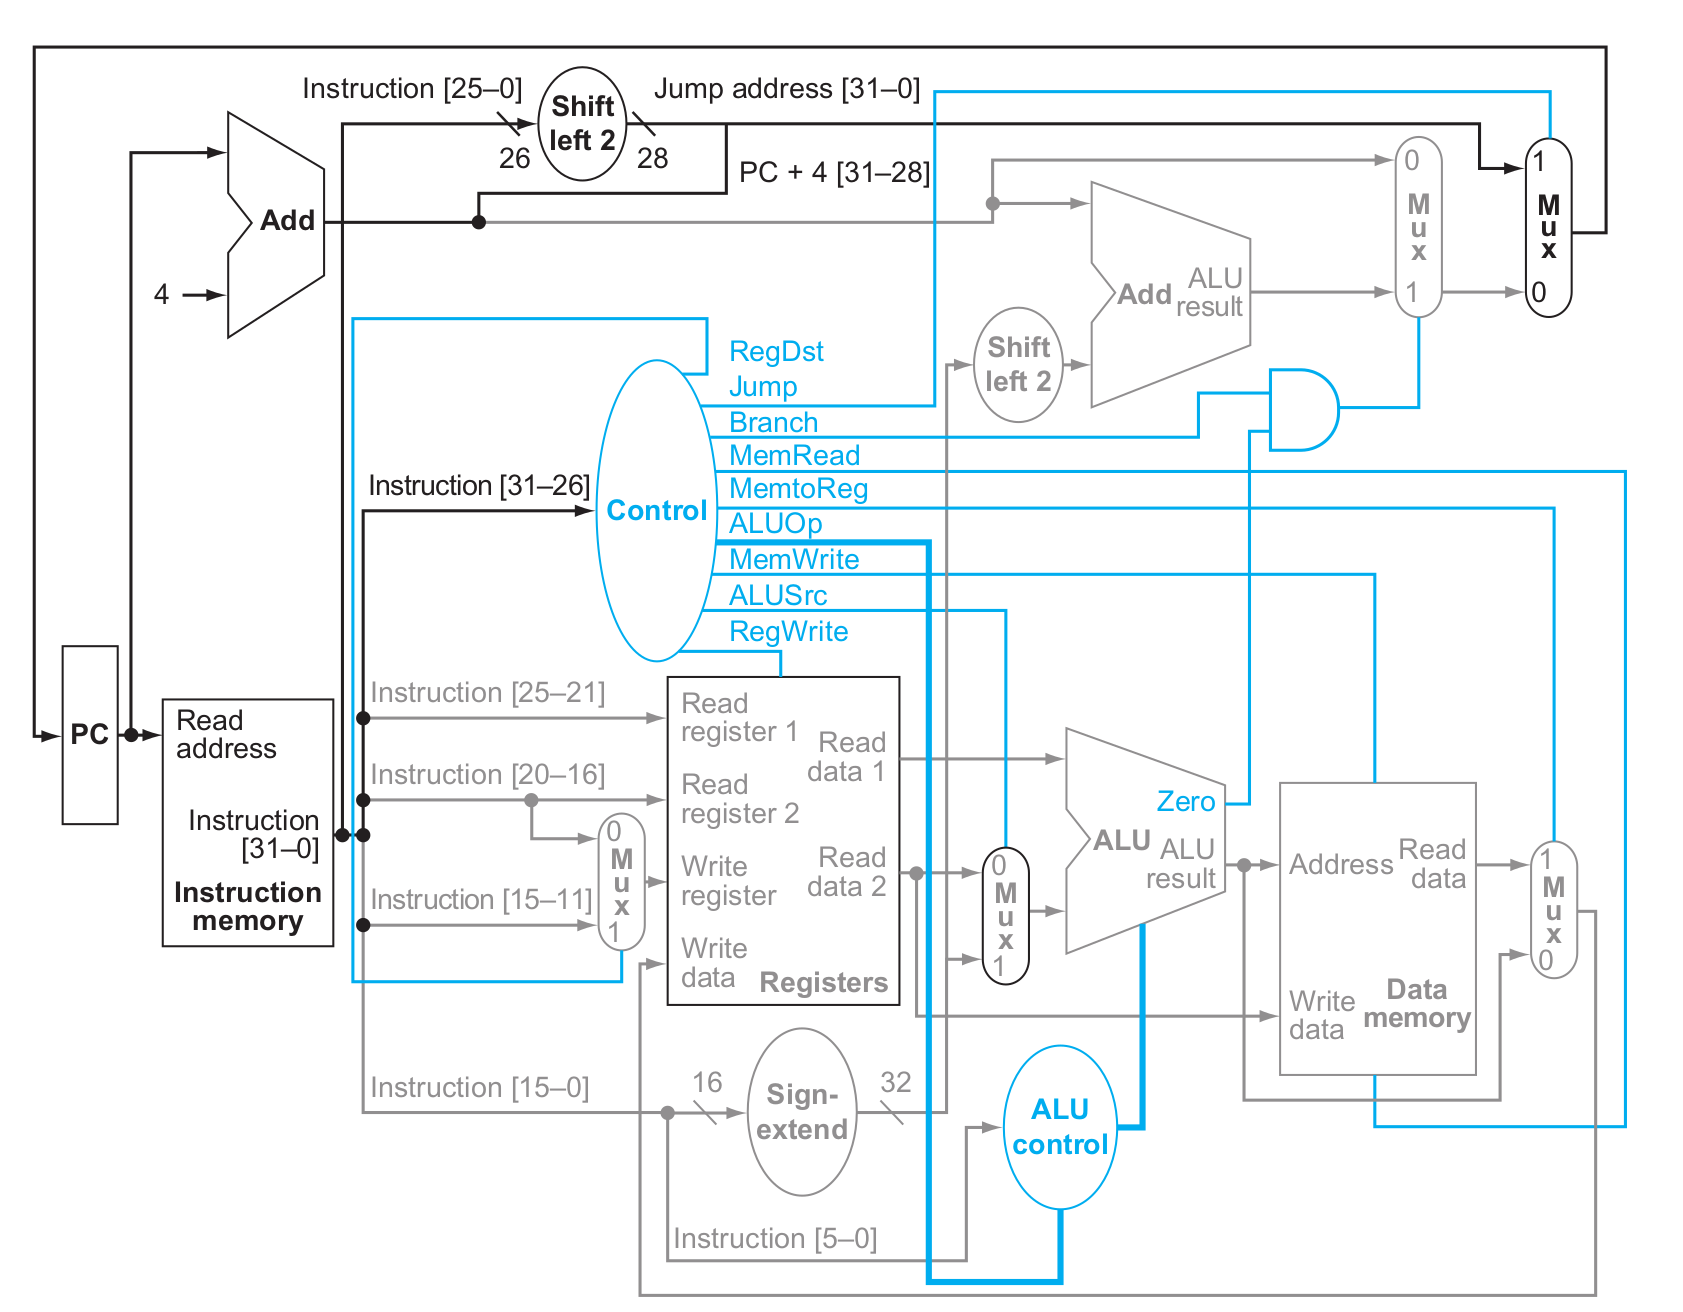
\includegraphics[width=0.9\columnwidth]{figs/datapath.png}
%\vspace{-12mm}
	\label{fig:datapath}
%\vspace{-5mm}
\end{figure}



\begin{parts}

\part[10] Explain the general flow of (\texttt{beq}) through the datapath. 

\newcommand{\beq}{\texttt{beq}}
\newcommand{\pc}{\texttt{PC}}

\textbf{Answer:} The datapath reads the \beq{} instruction from the instruction memory at the address 
contained in the \pc{} register. Bits [31-26] are read by the control unit to detect that this is a 
\beq{} instruction. Bits [25-21] and [20-16] select two registers from the register file. The values 
from these registers are routed to the ALU unit for comparison (note that the multiplexor controlled 
by the ALUSrc signal selects a register (deasserted). The control unit
	configures the ALU control unit to perform subtraction operation on the
	ALU. If register values are equal the Zero signal is asserted. 

The AND gate that takes Branch and Zero selects the final value of the \pc{}. In any case the \pc{} is already 
incremented by 4. If the Zero is deaserted the branch is not taken and the multiplexor selects this \pc{} + 4 
value for the next instruction. However if Zero is asserted, the multiplexor selects the value computed by 
another ALU, which is defined as a sum of \pc{} + 4 and by the bits [15-0] of the \beq{} instruction that are sign extended to 32 bits
and shifted by two. 


\vfill


	
\newpage
\part[5] Which control signals are asserted, i.e., true or 1. 
	

Control bits:

ALUSrc - deasserted
RegWrite - deasserted
RegDst - don't care
Jump - deasserted
Branch - asserted
Zero - asserted (if taken)
MemRead - deasserted
MemWrite - deasserted
MemtoReg - don't care

ALU Control bits are set for Bnegate, CarryIn and to select the addition operation. 


\vfill

\part[10] (and a badge of honor) The datapath has an error (with respect to how operation of the CPU was explained in Chapter 2 of the book). Find and explain the error. 

\textbf{Answer:} If you read the book carefully you will notice the following
	explanation for the \texttt{j} (jump) instruction: 

\begin{figure}[h] \centering
%\includegraphics[width=1.0\columnwidth]{figs/shared-state.png}
	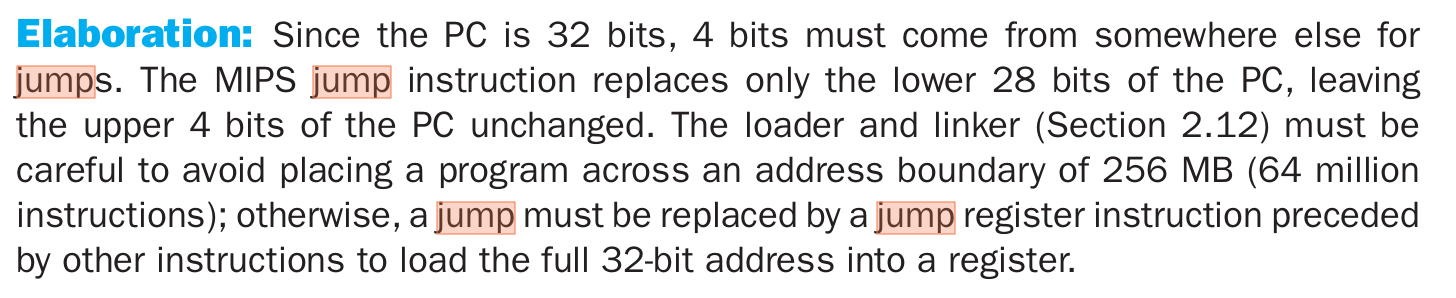
\includegraphics[width=0.7\columnwidth]{figs/jump.png}
%\vspace{-12mm}
	\label{fig:jump}
%\vspace{-5mm}
\end{figure} 
	
	
Specifically, \emph{``leaving the upper 4 bits of the PC unchanged''}.
Seemingly this hints that the datapath should concatenate the jump target (bits
[25-0] shifted by 2) with the \pc{} and not \pc{} + 4. And hance a different
wire in the datapath should exist. 

However, if you look at the MIPS specification
\url{https://www.cs.cornell.edu/courses/cs3410/2008fa/MIPS_Vol2.pdf} (page 115,
J instruction) you notice the following explanation: 

\emph{``The remaining upper bits are the corresponding bits of the address of
the instruction in the delay slot (not the branch itself)''}

I.e., really it's the upper bits of the next instruction or \pc{} + 4. So the
datapath seems to be correct with respect to the MIPS specification but
incorrect with respect to the earlier explanation in the book. 

Finally, note that the MIPS specification seems to have a bug in how it
explainst behavior of the jump instruction

\begin{figure}[h] \centering
%\includegraphics[width=1.0\columnwidth]{figs/shared-state.png}
	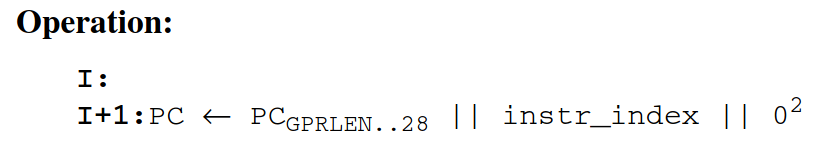
\includegraphics[width=0.5\columnwidth]{figs/jump-mips.png}
%\vspace{-12mm}
	\label{fig:jump-mips}
%\vspace{-5mm}
\end{figure} 
	
Specifically, it again mentions $PC_{GPRLEN..28}$ instead of $(PC
+4)_{GPRLEN..28}$, which is obscure. 

	

\vfill


\end{parts}





\end{questions}
%\afterpage{\null\newpage}
\afterpage{\null\newpage}
\end{document}
